\documentclass[11pt]{article}

\usepackage[margin=1in]{geometry}
\usepackage{amsmath,amssymb,amsthm,mathtools}
\usepackage{graphicx}
\usepackage{microtype}
\usepackage[hidelinks]{hyperref}
\usepackage{xcolor}

\newtheorem{theorem}{Theorem}
\newtheorem{lemma}[theorem]{Lemma}
\newtheorem{corollary}[theorem]{Corollary}
\newcommand{\D}{\mathbb D}
\newcommand{\T}{\mathbb T}
\newcommand{\N}{\mathbb N}
\newcommand{\ellA}{\ell_A^p}
\newcommand{\dd}{\,d}

\title{Embedding Measures for $\ell_A^p$ When $p>2$\\
\large A full candidate solution to the measure question in arXiv:2210.05823}
\author{Automated mathematics run \texttt{fa\_banach\_001}, lane 6}
\date{22 July 2026}

\begin{document}
\maketitle

\begin{center}
\fbox{\parbox{0.91\textwidth}{\textbf{Status.}
Full solution candidate, likely valid, awaiting human review.  The result
fully characterizes the norm inequality asked about at the end of
Cheng--Felder for every finite positive Borel measure, and hence for the
particular atomic measure in their equation (7.2).}}
\end{center}

\section{Source problem}

The source is R.~Cheng and C.~Felder, \emph{On Interpolation by Functions in
$\ell_A^p$}, arXiv:2210.05823 \cite{ChengFelder}.  For
$1<p<\infty$, the space $\ell_A^p$ consists of analytic functions
\[
 f(z)=\sum_{n=0}^{\infty}a_nz^n,\qquad
 \|f\|_{\ell_A^p}=\Big(\sum_{n=0}^{\infty}|a_n|^p\Big)^{1/p}.
\]
The source asks for a full characterization, when $2<p<\infty$, of its
equation (7.2), reproduced from page 27 below.

\begin{figure}[ht]
\centering
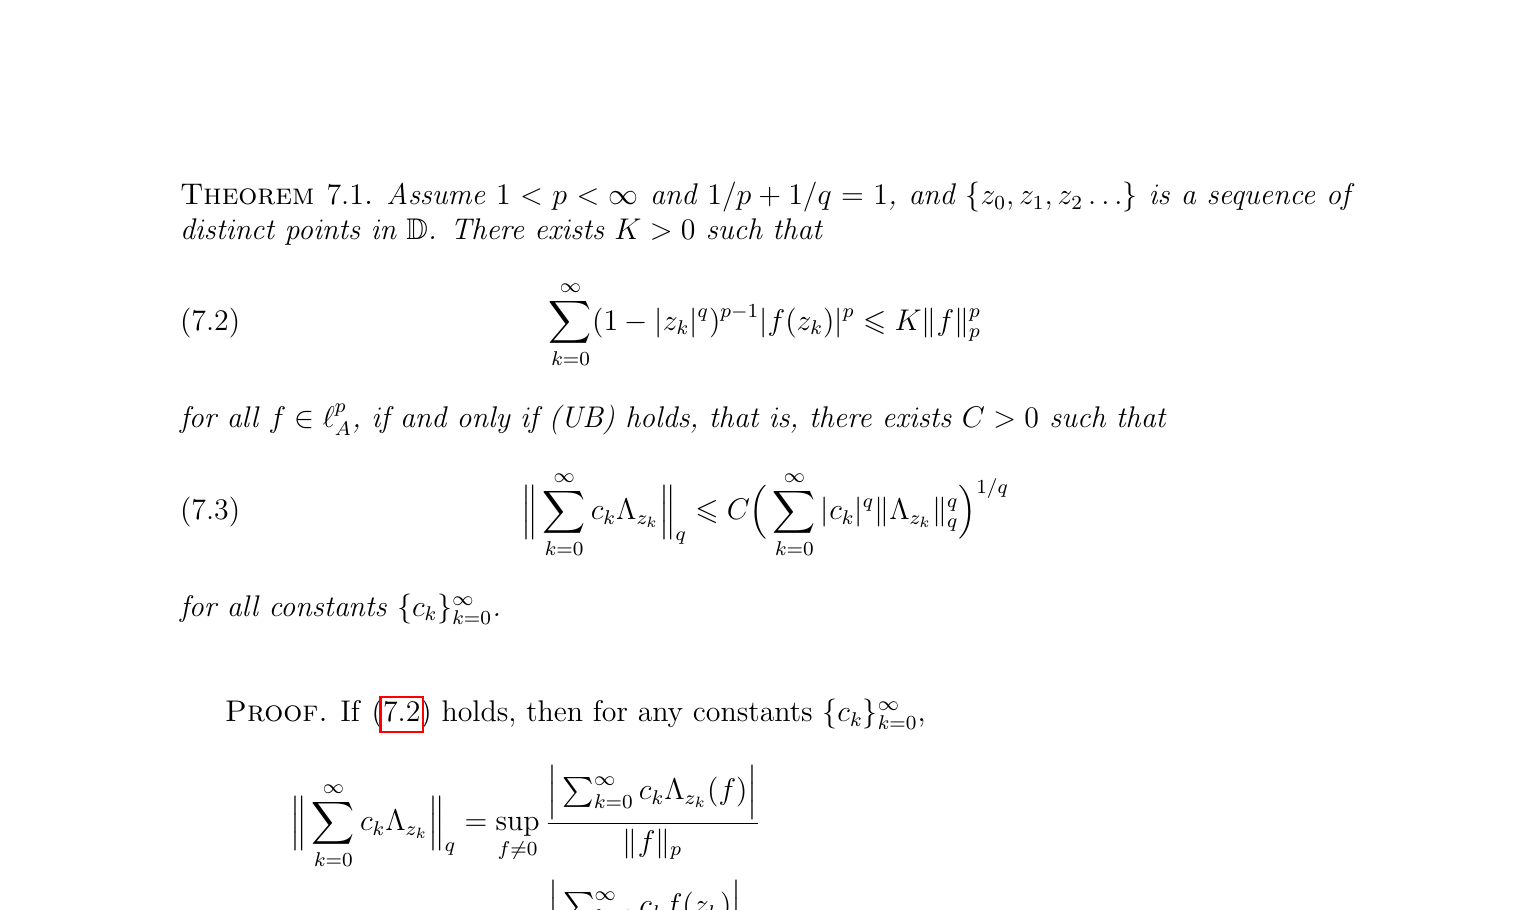
\includegraphics[width=0.98\textwidth]{figures/equation_7_2_crop.png}
\caption{Equation (7.2) and its interpretation in the source, page 27.}
\end{figure}

The closing question occurs on page 35.

\begin{figure}[ht]
\centering

\includegraphics[width=0.98\textwidth]{figures/open_question_crop.png}
\caption{The open question in the source, page 35.}
\end{figure}

In measure language, the problem is to characterize those finite positive
Borel measures $\mu$ on $\D$ for which
\begin{equation}\label{eq:embedding}
 \int_{\D}|f(z)|^p\dd\mu(z)\leq C\|f\|_{\ell_A^p}^p
 \qquad(f\in\ell_A^p).
\end{equation}
Indeed, equation (7.2) is \eqref{eq:embedding} for
\begin{equation}\label{eq:atomic-measure}
 \mu_Z=\sum_{k\geq0}(1-|z_k|^q)^{p-1}\delta_{z_k},
 \qquad \frac1p+\frac1q=1.
\end{equation}

For $0<h\leq1$ and $\theta\in\mathbb R$, write
\[
 S(\theta,h)=\{re^{it}\in\D:1-h\leq r<1,
 \ |t-\theta|\leq h/2\},
\]
with angles understood modulo $2\pi$.  Define
\[
 [\mu]_{p-1}=\sup_{\theta\in\mathbb R,\,0<h\leq1}
 \frac{\mu(S(\theta,h))}{h^{p-1}}.
\]

\section{Proof intuition}

The correct exponent can be read from a localized Dirichlet kernel.  A
polynomial with $N$ equal coefficients, normalized in $\ell^p$, has size
$N^{1-1/p}$ throughout a Carleson square of side comparable to $N^{-1}$.
If \eqref{eq:embedding} holds, that square can therefore carry mass at most
$N^{-(p-1)}$.

For the converse, the exponent $p-1$ identifies the right intermediate
space.  The weighted Bergman space with density $(1-|z|)^{p-3}$ has Carleson
exponent $(p-3)+2=p-1$.  A dyadic frequency calculation shows
\[
 \ell_A^p\hookrightarrow A^p_{p-3}.
\]
On a block of $N$ coefficients, the loss from $\ell^p$ coefficients to an
$L^p(\T)$ norm is $N^{1-2/p}$; its $p$-th power is $N^{p-2}$.  Radial
integration over the corresponding boundary layer contributes exactly
$N^{-(p-2)}$.  This cancellation is the core of the proof.  A standard
Whitney-box argument, included below, then embeds $A^p_{p-3}$ into
$L^p(\mu)$ precisely under the displayed box condition.

\section{Main theorem}

\begin{theorem}[Complete characterization]\label{thm:main}
Let $2<p<\infty$ and let $\mu$ be a finite positive Borel measure on $\D$.
Then \eqref{eq:embedding} holds for all $f\in\ell_A^p$ if and only if
$[\mu]_{p-1}<\infty$.  Quantitatively,
\[
 c_p[\mu]_{p-1}
 \leq
 \sup_{0\neq f\in\ell_A^p}
 \frac{\int_{\D}|f|^p\dd\mu}{\|f\|_{\ell_A^p}^p}
 \leq C_p[\mu]_{p-1},
\]
where $c_p,C_p>0$ depend only on $p$ (and on the harmless convention used
for Carleson squares).
\end{theorem}

\subsection*{Necessity}

Assume \eqref{eq:embedding} with best constant $M$.  Fix a square
$S(\theta,h)$ with $h$ small.  Choose an integer $N\asymp h^{-1}$ so that
$Nh\leq 1/16$, and put
\[
 F_{N,\theta}(z)=N^{-1/p}\sum_{n=0}^{N-1}e^{-in\theta}z^n.
\]
Its $\ell_A^p$ norm is one.  If $z=re^{i(\theta+t)}$ belongs to
$S(\theta,h)$, then $|t|\leq h/2$, $r\geq1-h$, and for $0\leq n<N$,
\[
 r^n\geq(1-h)^N\geq c,
 \qquad |nt|\leq Nh/2\leq1/32.
\]
Taking real parts after the rotation by $e^{-in\theta}$ gives
\[
 \left|\sum_{n=0}^{N-1}e^{-in\theta}z^n\right|\geq cN.
\]
Consequently $|F_{N,\theta}(z)|^p\geq c_pN^{p-1}$ throughout the square, and
\[
 M\geq\int_{\D}|F_{N,\theta}|^p\dd\mu
 \geq c_pN^{p-1}\mu(S(\theta,h)).
\]
Since $N\asymp h^{-1}$, this yields
$\mu(S(\theta,h))\leq C_pMh^{p-1}$.  For $h$ bounded away from zero, the
same conclusion follows by testing with the constant function $1$.  Hence
$[\mu]_{p-1}\leq C_pM$.

\subsection*{The critical coefficient-to-Bergman estimate}

Let $dA$ denote normalized area measure.

\begin{lemma}\label{lem:bergman}
For $2<p<\infty$ and every analytic polynomial
$f(z)=\sum a_nz^n$,
\begin{equation}\label{eq:critical-bergman}
 \int_{\D}|f(z)|^p(1-|z|)^{p-3}\dd A(z)
 \leq C_p\sum_{n\geq0}|a_n|^p.
\end{equation}
\end{lemma}

\begin{proof}
Set $\beta=1-2/p=(p-2)/p>0$.  Apart from the constant coefficient, split
$f$ into dyadic blocks
\[
 f_k(z)=\sum_{2^k\leq n<2^{k+1}}a_nz^n,
 \qquad b_k=\Big(\sum_{2^k\leq n<2^{k+1}}|a_n|^p\Big)^{1/p}.
\]
For a trigonometric polynomial $P$ with at most $N$ frequencies,
interpolation between
$\|P\|_\infty\leq N^{1/2}\|P\|_2$ and the identity on $L^2$ gives
\[
 \|P\|_p\leq N^{1/2-1/p}\|P\|_2.
\]
Applying this at radius $r$, and then using
$\|c\|_2\leq N^{1/2-1/p}\|c\|_p$, yields
\begin{equation}\label{eq:block}
 M_p(r,f_k)
 \leq C_p2^{k\beta}r^{2^k}b_k,
\end{equation}
where
$M_p(r,g)=(2\pi)^{-1/p}\|g(re^{it})\|_{L^p(0,2\pi)}$.

For $r\geq1/2$, let $j$ be determined by
$2^{-j-1}<1-r\leq2^{-j}$.  Since
$r^{2^k}\leq\exp(-c2^{k-j})$, Minkowski's inequality and
\eqref{eq:block} give
\[
 M_p(r,f)\leq |a_0|+C_pG_j,
 \qquad
 G_j=\sum_{k\geq0}2^{k\beta}e^{-c2^{k-j}}b_k.
\]
The radial weighted measure of this shell is comparable to
$2^{-j(p-2)}=2^{-j\beta p}$.  Moreover,
\begin{align*}
 2^{-j\beta}G_j
 &\leq
 \sum_{k\leq j}2^{-(j-k)\beta}b_k
 +\sum_{k>j}2^{(k-j)\beta}e^{-c2^{k-j}}b_k.
\end{align*}
Both right-hand kernels are summable as functions of $j-k$.  Young's
convolution inequality on $\ell^p(\mathbb Z)$ therefore shows
\[
 \sum_{j\geq1}2^{-j(p-2)}G_j^p
 \leq C_p\sum_{k\geq0}b_k^p.
\]
This proves \eqref{eq:critical-bergman} on $1/2\leq r<1$.  On
$0\leq r<1/2$, Holder's inequality gives
\[
 |f(re^{it})|
 \leq \|(a_n)\|_{\ell^p}
 \Big(\sum_{n\geq0}r^{np'}\Big)^{1/p'}
 \leq C_p\|(a_n)\|_{\ell^p},
\]
so the remaining part follows as well.
\end{proof}

\subsection*{The weighted Bergman Carleson step}

\begin{lemma}\label{lem:carleson}
Let $\alpha>-1$ and suppose a positive measure $\mu$ satisfies
\[
 \mu(S(\theta,h))\leq Kh^{\alpha+2}
 \qquad(0<h\leq1).
\]
Then every analytic $f$ satisfies
\begin{equation}\label{eq:bergman-carleson}
 \int_{\D}|f|^p\dd\mu
 \leq C_{p,\alpha}K
 \int_{\D}|f(z)|^p(1-|z|)^\alpha\dd A(z).
\end{equation}
\end{lemma}

\begin{proof}
Decompose a neighborhood of $\partial\D$ into dyadic Whitney boxes $Q$ of
angular and radial side length $h_Q$, and let $Q^*$ be a fixed enlargement.
Each $Q$ lies in a Carleson square of side comparable to $h_Q$, hence
$\mu(Q)\leq CKh_Q^{\alpha+2}$.  Since $|f|^p$ is subharmonic,
\[
 \sup_Q|f|^p
 \leq Ch_Q^{-2}\int_{Q^*}|f|^p\dd A
 \leq Ch_Q^{-\alpha-2}
 \int_{Q^*}|f(z)|^p(1-|z|)^\alpha\dd A(z).
\]
The last comparison is valid also for $-1<\alpha<0$, because
$1-|z|\asymp h_Q$ on $Q^*$.  Thus
\[
 \int_Q|f|^p\dd\mu
 \leq CK\int_{Q^*}|f(z)|^p(1-|z|)^\alpha\dd A(z).
\]
The enlarged boxes have bounded overlap.  Summing, and treating a fixed
central disk by the same submean estimate and the case $h=1$, proves
\eqref{eq:bergman-carleson}.
\end{proof}

\subsection*{Completion of the proof}

Assume $[\mu]_{p-1}<\infty$ and take $\alpha=p-3>-1$.  Since
$\alpha+2=p-1$, Lemma~\ref{lem:carleson} followed by
Lemma~\ref{lem:bergman} gives, for every analytic polynomial,
\[
 \int_{\D}|f|^p\dd\mu
 \leq C_p[\mu]_{p-1}
 \int_{\D}|f(z)|^p(1-|z|)^{p-3}\dd A(z)
 \leq C_p[\mu]_{p-1}\|f\|_{\ell_A^p}^p.
\]
For a general $f\in\ell_A^p$, its Taylor polynomials converge pointwise on
$\D$ and in $\ell_A^p$.  Fatou's lemma extends the same estimate to $f$.
Together with the necessity argument, this proves
Theorem~\ref{thm:main}. \qed

\section{The exact answer to equation (7.2)}

\begin{corollary}\label{cor:atomic}
Let $2<p<\infty$, $1/p+1/q=1$, and let $(z_k)$ be distinct points of $\D$.
The source inequality
\[
 \sum_{k\geq0}(1-|z_k|^q)^{p-1}|f(z_k)|^p
 \leq K\|f\|_{\ell_A^p}^p
\]
holds for every $f\in\ell_A^p$ if and only if
\begin{equation}\label{eq:packing}
 \sup_{\theta\in\mathbb R,\,0<h\leq1}
 h^{-(p-1)}
 \sum_{z_k\in S(\theta,h)}(1-|z_k|^q)^{p-1}<\infty.
\end{equation}
\end{corollary}

\begin{proof}
If the source inequality holds, testing with the constant function shows that
the atomic measure~\eqref{eq:atomic-measure} is finite.  Conversely,
condition~\eqref{eq:packing}, together with a finite covering of the disk by
Carleson squares of side one, also implies finiteness.  The assertion now
follows by applying Theorem~\ref{thm:main} to that atomic measure.
\end{proof}

Thus the open norm inequality is characterized by an explicit
$(p-1)$-Carleson packing condition.  The ordinary Carleson condition found in
the source is weaker, exactly as its counterexample indicates.

\section{Verification and novelty check}

\paragraph{Internal verification.}
The proof is scale-invariant at both decisive points.  A normalized block of
$N$ equal coefficients has boundary $L^p$ size $N^{1-2/p}$, whose $p$-th
power is $N^{p-2}$; the weight $(1-r)^{p-3}\dd r$ assigns mass
$N^{-(p-2)}$ to the layer $1-r\asymp N^{-1}$.  The diagnostic script
\texttt{code/check\_scaling.py} samples the Dirichlet lower bound and checks
this exponent cancellation for $p=2.2,2.5,3,4,6$ and
$N=8,16,32,64,128$.  These computations are sanity checks, not proof.

\paragraph{Bounded literature search.}
On 22 July 2026 we searched the run indexes and web/arXiv results for
\texttt{2210.05823}, ``$\ell_A^p$ Carleson measure'', ``analytic coefficient
space $\ell^p$ Carleson'', ``$p-3$ weighted Bergman $\ell^p$ coefficients'',
and the proposed exponent ``$|I|^{p-1}$''.  The search found the source paper
and general weighted Bergman Carleson theorems, but no paper stating the
characterization in Theorem~\ref{thm:main} or Corollary~\ref{cor:atomic}.
This is a bounded, not exhaustive, novelty check.

\paragraph{Limitations and reviewer focus.}
The packet addresses the measure/norm-inequality question and therefore the
source condition (UB) through Theorem 7.1 of the source.  It does not settle
the separate requested connection between weak separation and condition (LB),
nor questions about other uses of the nonlinear Gramian.  The main review
point is Lemma~\ref{lem:bergman}, especially the negative but integrable weight
$p-3\in(-1,0)$ when $2<p<3$.

\paragraph{Recommendation.}
Send for expert review as a full solution candidate to the explicit norm
inequality (7.2).  If accepted, the natural next step is to state the packing
condition directly as a characterization of (UB) and investigate whether it
interacts with the source's weak-separation conditions.

\begin{thebibliography}{9}

\bibitem{ChengFelder}
R.~Cheng and C.~Felder,
\emph{On Interpolation by Functions in $\ell_A^p$},
arXiv:2210.05823, 2022.

\bibitem{DurenSchuster}
P.~Duren and A.~Schuster,
\emph{Bergman Spaces},
Mathematical Surveys and Monographs 100, American Mathematical Society, 2004.

\end{thebibliography}

\end{document}
